\chapter{System Architecture}
\label{chap:architecture}
\section{Threat Model}
In this work, we assume the adversary aims specifically to bring our simulated infrastructure down using a volumetric DDoS attack, in either TCP SYN Flood or UDP Flood. We also assume that the attacker controls a botnet which wasn't blocked or flagged beforehand, so other security appliances will not intervene to thwart this attack.

The network medium for the software side is a virtual network, made using VirtualBox's network driver, and also the Docker Network stack. To connect these virtualized networks, we are using a 1Gbps capable SOHO router, to which the IoT target device is connected to. A maximum of 65535 bots will be simulated through the virtualized environment, taking up a whole /16 subnet. We consider the botnet size to be adequate, given that the infamous Mirai botnet had a peak of an estimated 600.000 devices\cite{antonakakis2017}, as we consider comparable sizes of botnets to be more frequent. Also, we expect the attacker to be able to generate up to 1Gbps of traffic in total, as the network is expected to impose bandwidth limitations regardless.

The attacker generates the 1Gbps traffic using the Ixia Breakingpoint traffic generator appliance, with the specific traffic curve shown in \autoref{fig:data-rate}\cite{vladescu2025}.

\begin{figure}
    \centering
    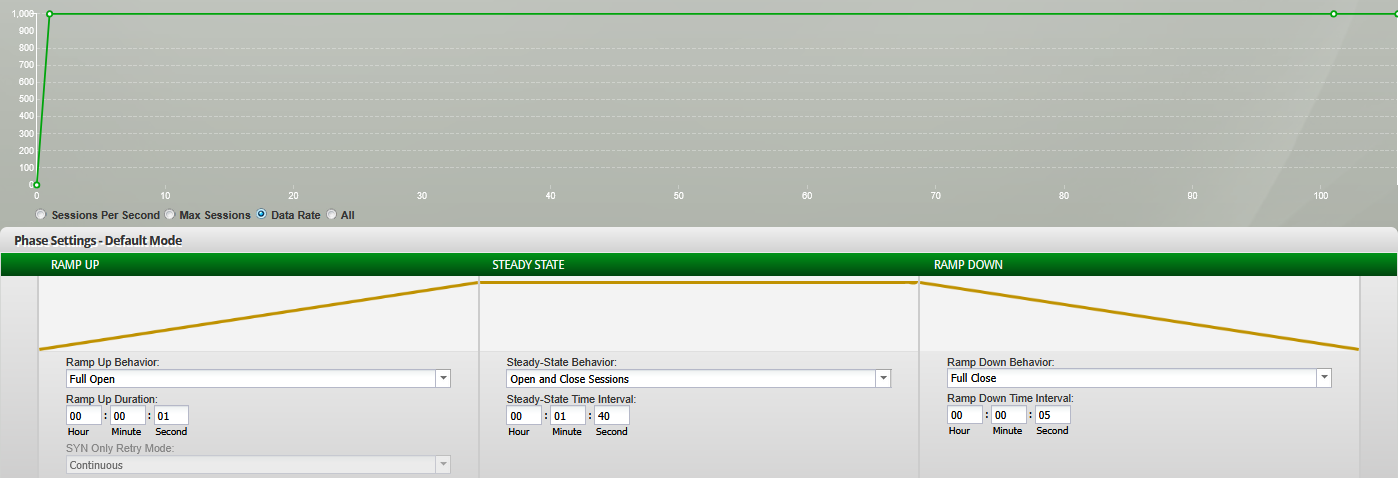
\includegraphics[width=1\linewidth]{images/breakingpoint_curve.png}
    \caption{Ixia Packet Generator Data Rate Curve}
    \label{fig:data-rate}
\end{figure}


The control plane between the SDN components are not a target for this scenario, and also other attacks that aim to disrupt by hijacking the infrastructure itself are not the aim of this work.
The two scenarios being tested are as follows in the next subsections.

\subsection{DDoS flood before being connected}
This case is a standard in the case of DDoS botnets, and is differentiated by the fact that the bots will not try to connect to the system through conventional methods, such as querying the authoritative DNS server, but will try to flood directly to the IP which is obtained by a scanner bot.

\subsection{DDoS flood after being connected}
This is an edge case, when the botnet manages to query the authoritative DNS server, without triggering any security alarm, or DoS detection. In this case, the DDoS is going to hit the returned IP from the DNS server, and the protection is more exposed.

\section{Architecture Overview}

The backbone of the system is structured as such:
\begin{itemize}
    \setlength\itemsep{1pt}
    \setlength\topsep{1pt}
    \setlength\parsep{1pt}
    \setlength\parskip{1pt}
    \item Master node
    \item Proxy node(s)
    \item Nest node(s)
    \item IoT device(s)
\end{itemize}

\autoref{img:arch}\cite{vladescu2025} shows how these components are pieced together, and how they interact on an infrastructural level.

\begin{figure}[ht]
    \centering
    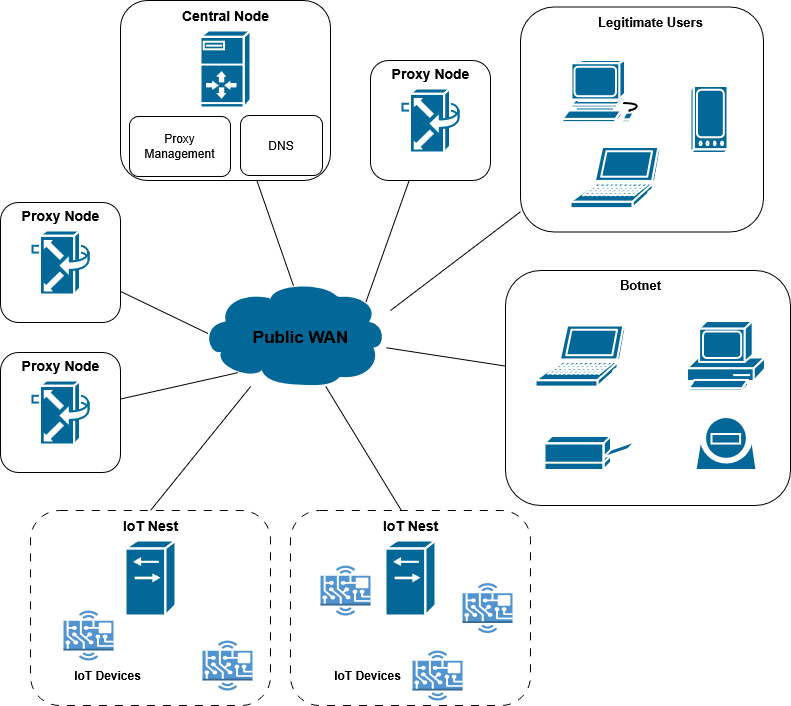
\includegraphics[width=0.75\linewidth]{images/system_architecture.png}
    \caption{System architecture}
    \label{img:arch}
\end{figure}

Starting hierarchically, the master node is what can be considered an SDN controller, since it incorporates the program that manages proxies through the southband MQTT protocol, and in addition handles DNS requests with the help of an embedded DNS server. This master node is considered unique in the system.

The proxy nodes serve as the foundational layer of abstraction between the clients and IoT servers. They conceal the IoT networks and permit only traffic that has been independently approved by the master node. Two proxies may not exist in the same configuration, since their routing tables will not contain any common client-nest pairs. The routing stack configuration is done through nftables, and each proxy perform NAT masquerade, with DNAT and SNAT.

Nest nodes are the final destination between a client's packets and the IoT device. They are configured to accept and forward traffic only from the approved proxies, and serve as the gateway of the IoT LAN. In a more realistic scenario, this gateway may be swapped with a regular IoT gateway/edge router, since IoT devices are known for using IoT-specific transmitting mediums, such as Z-Wave, Thread, Matter, Zigbee, Bluetooth, in the case of consumer IoT devices, or Modbus over IP, RS-485 in industrial/SCADA devices.

The target IoT device being tested is an Espressif ESP8266 development board. We consider this MCU an equivalent for most of the devices on the market as of the time of writing this thesis, and has the following characteristics: 32bit single core Tensilica L106, running at either 80 or 160MHz, and uses the built-in WiFi driver to connect to our nest node gateway. To simulate the service, we are using a combination of temperature reading from the built-in sensor, using the ADC, combined with a generated random number. All of this is hashed using SHA2 256, using calls to the cryptographic engine of the ESP8266 SoC. We believe this is a fair computational workload, since it uses composite resource access, complete with the HTTP server running in a separate FreeRTOS thread.


\section{Proposed Algorithm}

An initial DNS query will take place, before the client may access any resource on the Internet, as it is normal. The recursive DNS server will redirect the query to the autorithative DNS server, embedded in the master node, and this query marks the initial step of our algorithm. When the client $C$, using it's ephemeral IP from the ISP, $C_{IP_K}$ requests the IP of the service of our controlled domain, $D$, the recursive DNS server will evenutally lead to the DNS held by our system, the defender side. The master node will then make a decision based on the reputation of the connecting client's IP, if he's been marked before or not. In the case of a "clean" client, it will forward an IP of one of the proxies. The algorithm is also described in \autoref{alg:dns-resolution}\cite{vladescu2025}.

\begin{algorithm}[ht]
    \caption{DNS Resolution with Proxy Assignment and SDN Integration}
    \label{alg:dns-resolution}
    \LinesNotNumbered      % Turn off line numbers (if they were on)
    %\SetAlgoLined          % (Optional) if you want horizontal lines at each block—though you can also omit this
    \KwResult{Client connects to IoT Device}
    \vspace{6pt}
    $C_{IP_K} \xrightarrow{DNS Query} S_k$\;
    \vspace{2pt}
    $DNS \xrightarrow{IP_K} M_{SDN}$\;
    \vspace{2pt}
    \eIf{$IP_K \notin IP_{Blacklist}$}{
    \eIf{$IP_K \in \{\,IP_{Client} \mid (IP_K,IP_{Proxy}) \in P_{Assigned}\}$}{
      \Return{$IP_{Proxy} \mid (IP_K,IP_{Proxy}) \in P_{Assigned}$}
    }{
      Choose $IP_{Proxy} \sim \text{Random}(\mathcal{P})$\;
      Add $(IP_K,IP_{Proxy})$ to $P_{Assigned}$\;
      \Return{$IP_{Proxy}$}
    }
    }{
    Close connection\;
    }
\end{algorithm}

The end result of this algorithm is the client is allowed on the system, and is given the IP of the proxy tied to the final nest gateway. The designated proxy will have been modified by the master node through the MQTT southbount API to allow the traffic through iptables rules with DNAT and SNAT.

\begin{figure}
    \centering
    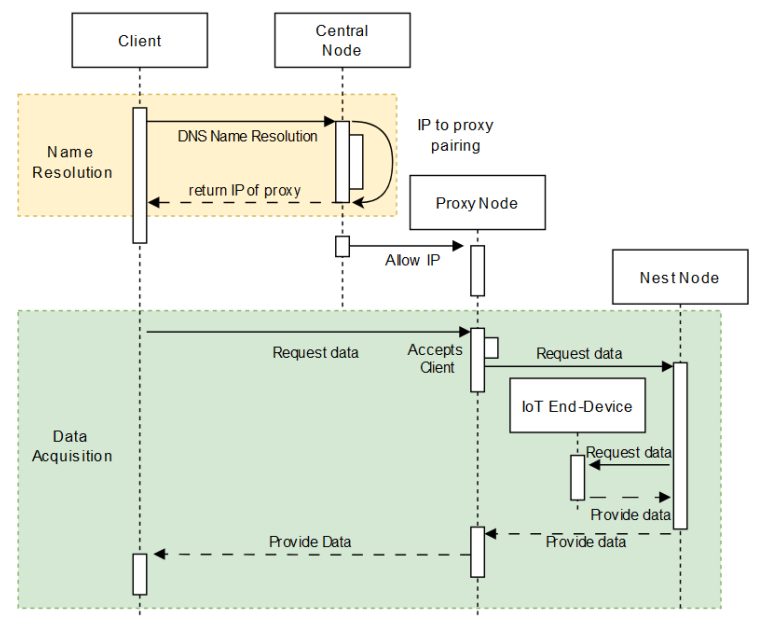
\includegraphics[width=0.7\linewidth]{images/sequence_diagram.png}
    \caption{Sequence diagram of the connection and data flow}
    \label{img:seq-diag}
\end{figure}

After this connection steps, the client may request data from the IoT server seamlessly, as shown in \autoref{alg:data-flow}\cite{vladescu2025}. Using regular HTTP, for example, he will first make a TCP three-way handshake, but with the proxy, not with the IoT. The IP masquarade will be an opaque wall from the point of view of the IoT nest and the client. After the TCP handshake, the two entities may exchange data on HTTP seamlessly, with an added delay of another hop, practically, since the traffic is relayed. A good way of visualising the whole connection algorithm and data exchange is expressed in \autoref{img:seq-diag}\cite{vladescu2025}, where the yellow part is the connection phase, and the green segment is the data transfer.

\begin{algorithm}[ht]
    \caption{Client-Server Communication Dataflow}
    \label{alg:data-flow}
    \LinesNotNumbered
    \KwResult{Client retrieves data from IoT Device}
    \vspace{6pt}
    $C_{IP_K} \xrightarrow{\text{GET Request}} P_{IP_{Proxy}}$\;
    \vspace{4pt}
    \eIf{$IP_K \in P_{Allowed}$}{
        \vspace{2pt}
        $NAT(IP_K \to IP_{Proxy}, IP_{Proxy} \to IP_{Nest})$\;
        $IP_{Nest} \iff IP_{IoT}$\;
    }{
        Close connection\;
    }
\end{algorithm}

A DDoS attack is expressed in \autoref{alg:attack-flow}\cite{vladescu2025}, where the number of requests, $R$, is measured with a fixed or dynamic threshold, $R_{th}$. $R$ is computed as the number of requests in a period of time, $\frac{N_{req}(T)}{T}$. If the threshold is bigger, then a series of events happen: the SDN master node, $M_{SDN}$, will receive a DDoS alert from the proxy, signaling it will need a new IP address from the ISP. Also, the offending IPs are added to the master node's blacklist, so that the DNS will not forward them an available proxy IP. After receiving a new IP, the service will restart itself.

\begin{algorithm}[ht]
    \caption{Handling of an Attack Through Naive Detection}
    \label{alg:attack-flow}
    %\SetAlgoLined
    \KwResult{Attacker is interrupted proactively}
    \vspace{6pt}
    \While{Proxy Server Active}{
    \State $R \gets \frac{N_{req}(T)}{T}$ \;
    \vspace{4pt}
            \If{$R > R_{th}$}{
            \State $ M_{SDN} \xleftarrow[Renew IP]{\text{DDoS Attempt}}Proxy$\;
            \vspace{6pt}
            \State  $M_{\mathrm{SDN}} \xleftarrow[\text{Blacklist Update}]{\mathrm{IP}_{\mathrm{offending}}}Proxy$\;
            \vspace{6pt}
            \State $M_{SDN} \xrightarrow[Provider API]{\text{Request new IP}} ISP$ \;
            \vspace{6pt}
            \State $IP_{Proxy_{Old}} \xleftarrow{\text{Replace}} IP_{Proxy_{New}}$
        }
        \EndIf
    }
    \EndWhile{}
\end{algorithm}
